\documentclass[tikz,border=12pt]{standalone}
\usepackage{amsmath,amssymb}
\usetikzlibrary{positioning,fit,backgrounds,arrows.meta,calc}


\definecolor{cGrn}{RGB}{34,120,56}     % backbone (global, shared)
\definecolor{cBlu}{RGB}{30,100,200}    % global attention (FedAvg)
\definecolor{cOra}{RGB}{200,80,20}     % local attention (per-client)
\definecolor{cGry}{RGB}{70,70,80}      % I/O boxes, server

% ---------------------------------------------------------------------------
% TikZ styles
% ---------------------------------------------------------------------------
\tikzset{
  %── Architecture nodes ────────────────────────────────────────────────────
  io/.style={
    draw=cGry, fill=gray!12, rounded corners=3pt,
    text centered, font=\footnotesize\sffamily,
    minimum width=3.8cm, minimum height=0.60cm, inner sep=3pt},
  bb/.style={
    draw=cGrn, fill=cGrn!12, rounded corners=3pt,
    text centered, font=\footnotesize\sffamily,
    minimum width=3.8cm, minimum height=0.55cm, inner sep=2pt},
  ga/.style={
    draw=cBlu, fill=cBlu!12, rounded corners=2pt,
    text centered, font=\scriptsize\sffamily,
    minimum width=1.75cm, minimum height=0.72cm, inner sep=2pt},
  la/.style={
    draw=cOra, fill=cOra!12, rounded corners=2pt,
    text centered, font=\scriptsize\sffamily,
    minimum width=1.75cm, minimum height=0.72cm, inner sep=2pt},
  cb/.style={
    draw=gray!55, fill=gray!7, rounded corners=2pt,
    text centered, font=\scriptsize\sffamily,
    minimum width=3.8cm, minimum height=0.45cm, inner sep=2pt},
  dualframe/.style={
    draw=black!40, fill=yellow!5,
    rounded corners=5pt, inner sep=5pt,
    dashed, line width=0.7pt},
  %── FL diagram nodes ──────────────────────────────────────────────────────
  sv/.style={
    draw=cGry!80, fill=cGry!10, rounded corners=5pt,
    minimum width=8.0cm, minimum height=1.0cm,
    text centered, font=\small\sffamily, inner sep=5pt},
  cl/.style={
    draw=cBlu!70, fill=cBlu!8, rounded corners=4pt,
    minimum width=1.75cm, minimum height=1.0cm,
    text centered, font=\scriptsize\sffamily, inner sep=4pt},
  gp/.style={
    draw=cBlu!70, fill=cBlu!8, rounded corners=3pt,
    font=\scriptsize\sffamily, inner sep=4pt,
    text width=3.4cm, text centered},
  lp/.style={
    draw=cOra!80, fill=cOra!8, rounded corners=3pt,
    font=\scriptsize\sffamily, inner sep=4pt,
    text width=3.2cm, text centered},
  %── Arrows ────────────────────────────────────────────────────────────────
  va/.style={-{Stealth[length=5pt,width=3.5pt]},
             line width=0.9pt, draw=black!60},
  da/.style={-{Stealth[length=5pt,width=3.5pt]},
             line width=1.2pt, draw=cBlu!80},
  ua/.style={-{Stealth[length=5pt,width=3.5pt]},
             line width=1.2pt, draw=cOra!90},
}

% ---------------------------------------------------------------------------
\begin{document}
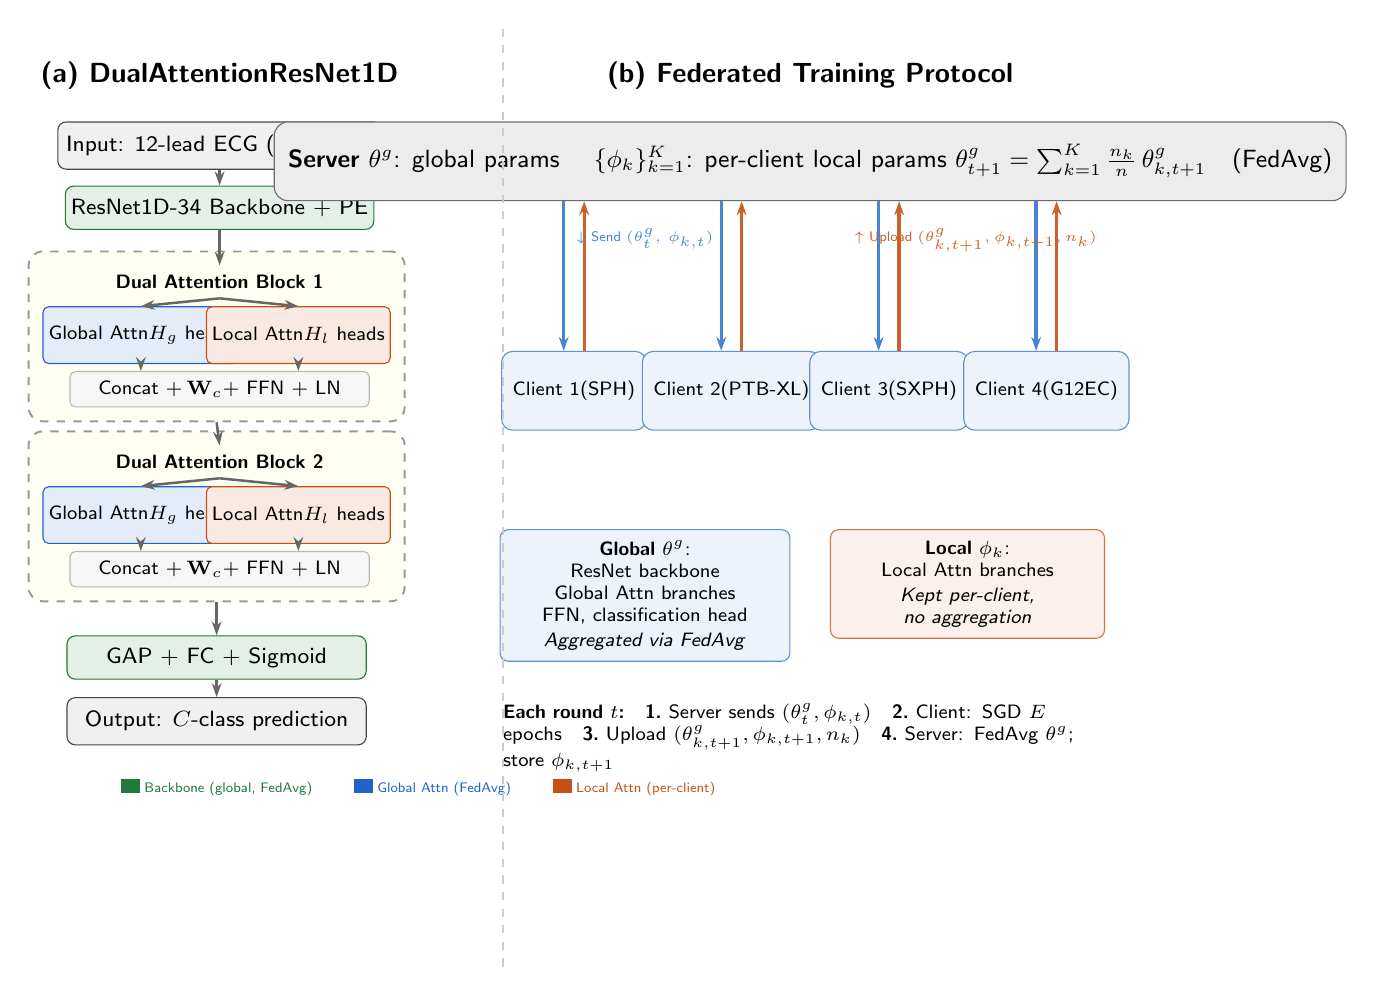
\begin{tikzpicture}

% =============================================================================
% LEFT PANEL: DualAttentionResNet1D Architecture
% =============================================================================

% Panel title
\node[font=\normalsize\bfseries\sffamily] (ltitle) at (0, 0)
  {(a) DualAttentionResNet1D};

% I/O
\node[io, below=0.28cm of ltitle] (input)
  {Input: 12-lead ECG ($12{\times}5000$)};

% Collapsed backbone (Conv stem + 4 ResNet stages + PE)
\node[bb, below=0.20cm of input] (backbone)
  {ResNet1D-34 Backbone $+$ PE};

% -------------------------------------------------
% Dual Attention Block 1
% -------------------------------------------------
\node[font=\scriptsize\bfseries\sffamily, below=0.45cm of backbone]
  (da1lbl) {Dual Attention Block 1};

\node[ga, below=0.10cm of da1lbl, xshift=-1.0cm] (g1)
  {Global Attn\\$H_g$ heads};

\node[la, below=0.10cm of da1lbl, xshift=+1.0cm] (l1)
  {Local Attn\\$H_l$ heads};

\node[cb] at ($(g1.south)!0.5!(l1.south)+(0,-0.32)$) (cb1)
  {Concat $+\,\mathbf{W}_c +$ FFN $+$ LN};

\begin{scope}[on background layer]
  \node[dualframe, fit=(da1lbl)(g1)(l1)(cb1)] (da1) {};
\end{scope}

% -------------------------------------------------
% Dual Attention Block 2
% -------------------------------------------------
\node[font=\scriptsize\bfseries\sffamily, below=0.48cm of cb1]
  (da2lbl) {Dual Attention Block 2};

\node[ga, below=0.10cm of da2lbl, xshift=-1.0cm] (g2)
  {Global Attn\\$H_g$ heads};

\node[la, below=0.10cm of da2lbl, xshift=+1.0cm] (l2)
  {Local Attn\\$H_l$ heads};

\node[cb] at ($(g2.south)!0.5!(l2.south)+(0,-0.32)$) (cb2)
  {Concat $+\,\mathbf{W}_c +$ FFN $+$ LN};

\begin{scope}[on background layer]
  \node[dualframe, fit=(da2lbl)(g2)(l2)(cb2)] (da2) {};
\end{scope}

% Collapsed classifier head (GAP + FC + Sigmoid)
\node[bb, below=0.42cm of da2] (head)
  {GAP $+$ FC $+$ Sigmoid};

\node[io, below=0.22cm of head] (out)
  {Output: $C$-class prediction};

% ------ Left-panel arrows -----------------------------------------------
\draw[va] (input) -- (backbone);
\draw[va] (backbone.south) -- (da1lbl.north);
\draw[va] (da1lbl.south) -- (g1.north);
\draw[va] (da1lbl.south) -- (l1.north);
\draw[va] (g1.south) -- (cb1.north -| g1);
\draw[va] (l1.south) -- (cb1.north -| l1);
\draw[va] (da1.south) -- (da2lbl.north);
\draw[va] (da2lbl.south) -- (g2.north);
\draw[va] (da2lbl.south) -- (l2.north);
\draw[va] (g2.south) -- (cb2.north -| g2);
\draw[va] (l2.south) -- (cb2.north -| l2);
\draw[va] (da2.south) -- (head.north);
\draw[va] (head) -- (out);

% Color key (bottom of left panel)
\node[font=\tiny\sffamily, below=0.30cm of out, color=cGrn]
  (key1) {\rule{7pt}{5pt}\;Backbone (global, FedAvg)};
\node[font=\tiny\sffamily, right=0.28cm of key1, color=cBlu]
  (key2) {\rule{7pt}{5pt}\;Global Attn (FedAvg)};
\node[font=\tiny\sffamily, right=0.28cm of key2, color=cOra]
  {\rule{7pt}{5pt}\;Local Attn (per-client)};


% =============================================================================
% RIGHT PANEL: Federated Learning Protocol
% =============================================================================

% Panel title — aligned to top of left panel, offset right
\node[font=\normalsize\bfseries\sffamily]
  at ([xshift=7.5cm]ltitle) (rtitle)
  {(b) Federated Training Protocol};

% Server box
\node[sv, below=0.28cm of rtitle] (srv)
  {\textbf{Server}\\[2pt]
   $\theta^{g}$: global params \quad
   $\{\phi_k\}_{k=1}^{K}$: per-client local params\\[1pt]
   $\theta^{g}_{t+1} = \sum_{k=1}^{K}
     \frac{n_k}{n}\,\theta^{g}_{k,t+1}$\quad(FedAvg)};

% 4 client boxes — closer to server
\node[cl, below=1.9cm of srv, xshift=-3.0cm] (c1)
  {Client 1\\(SPH)};
\node[cl, below=1.9cm of srv, xshift=-1.0cm] (c2)
  {Client 2\\(PTB-XL)};
\node[cl, below=1.9cm of srv, xshift=+1.0cm] (c3)
  {Client 3\\(SXPH)};
\node[cl, below=1.9cm of srv, xshift=+3.0cm] (c4)
  {Client 4\\(G12EC)};

% ------ Down arrows (server → clients, blue) --------------------------------
\draw[da] ($(srv.south -| c1)+(-0.13,0)$) -- ($(c1.north)+(-0.13,0)$);
\draw[da] ($(srv.south -| c2)+(-0.13,0)$) -- ($(c2.north)+(-0.13,0)$);
\draw[da] ($(srv.south -| c3)+(-0.13,0)$) -- ($(c3.north)+(-0.13,0)$);
\draw[da] ($(srv.south -| c4)+(-0.13,0)$) -- ($(c4.north)+(-0.13,0)$);

% ------ Up arrows (clients → server, orange) --------------------------------
\draw[ua] ($(c1.north)+(+0.13,0)$) -- ($(srv.south -| c1)+(+0.13,0)$);
\draw[ua] ($(c2.north)+(+0.13,0)$) -- ($(srv.south -| c2)+(+0.13,0)$);
\draw[ua] ($(c3.north)+(+0.13,0)$) -- ($(srv.south -| c3)+(+0.13,0)$);
\draw[ua] ($(c4.north)+(+0.13,0)$) -- ($(srv.south -| c4)+(+0.13,0)$);

% Arrow labels
\node[font=\tiny\sffamily, color=cBlu!80,
      below=0.22cm of srv, xshift=-2.1cm, align=center]
  {$\downarrow$ Send $(\theta^{g}_{t},\,\phi_{k,t})$};

\node[font=\tiny\sffamily, color=cOra!90,
      below=0.22cm of srv, xshift=+2.1cm, align=center]
  {$\uparrow$ Upload $(\theta^{g}_{k,t+1},\phi_{k,t+1},n_k)$};

% ------ Parameter partition boxes -------------------------------------------
\coordinate (cli4mid) at ($(c1.south)!0.5!(c4.south)$);

\node[gp, anchor=north east] at ($(cli4mid)+(-0.25,-1.25)$) (gbox)
  {\textbf{Global} $\theta^{g}$:\\
   ResNet backbone\\
   Global Attn branches\\
   FFN, classification head\\[1pt]
   \textit{Aggregated via FedAvg}};

\node[lp, anchor=north west] at ($(cli4mid)+(+0.25,-1.25)$) (lbox)
  {\textbf{Local} $\phi_k$:\\
   Local Attn branches\\[1pt]
   \textit{Kept per-client,\\no aggregation}};

% ------ Communication steps (below param boxes) -----------------------------
\coordinate (parambot) at ($(gbox.south west)!0.5!(lbox.south east)+(0,-0.55)$);
\node[font=\scriptsize\sffamily, anchor=north,
      text width=7.6cm, align=left] at (parambot) (steps)
  {\textbf{Each round $t$:}\quad
   \textbf{1.}~Server sends $(\theta^{g}_{t},\phi_{k,t})$\quad
   \textbf{2.}~Client: SGD $E$ epochs\quad
   \textbf{3.}~Upload $(\theta^{g}_{k,t+1},\phi_{k,t+1},n_k)$\quad
   \textbf{4.}~Server: FedAvg $\theta^{g}$; store $\phi_{k,t+1}$};

% =============================================================================
% Dividing line between panels
% =============================================================================
\coordinate (divtop) at ($(ltitle.north east)!0.5!(rtitle.north west)+(0,0.3)$);
\draw[gray!40, dashed, line width=0.6pt] (divtop) -- ++(0,-12);

\end{tikzpicture}
\end{document}
